% Source ownership:
% - Arthur: results and analysis


\section{Parallel Simulation Results}\label{sec:parallel-simulation-results}

\begin{figure}[H]
  \centering
  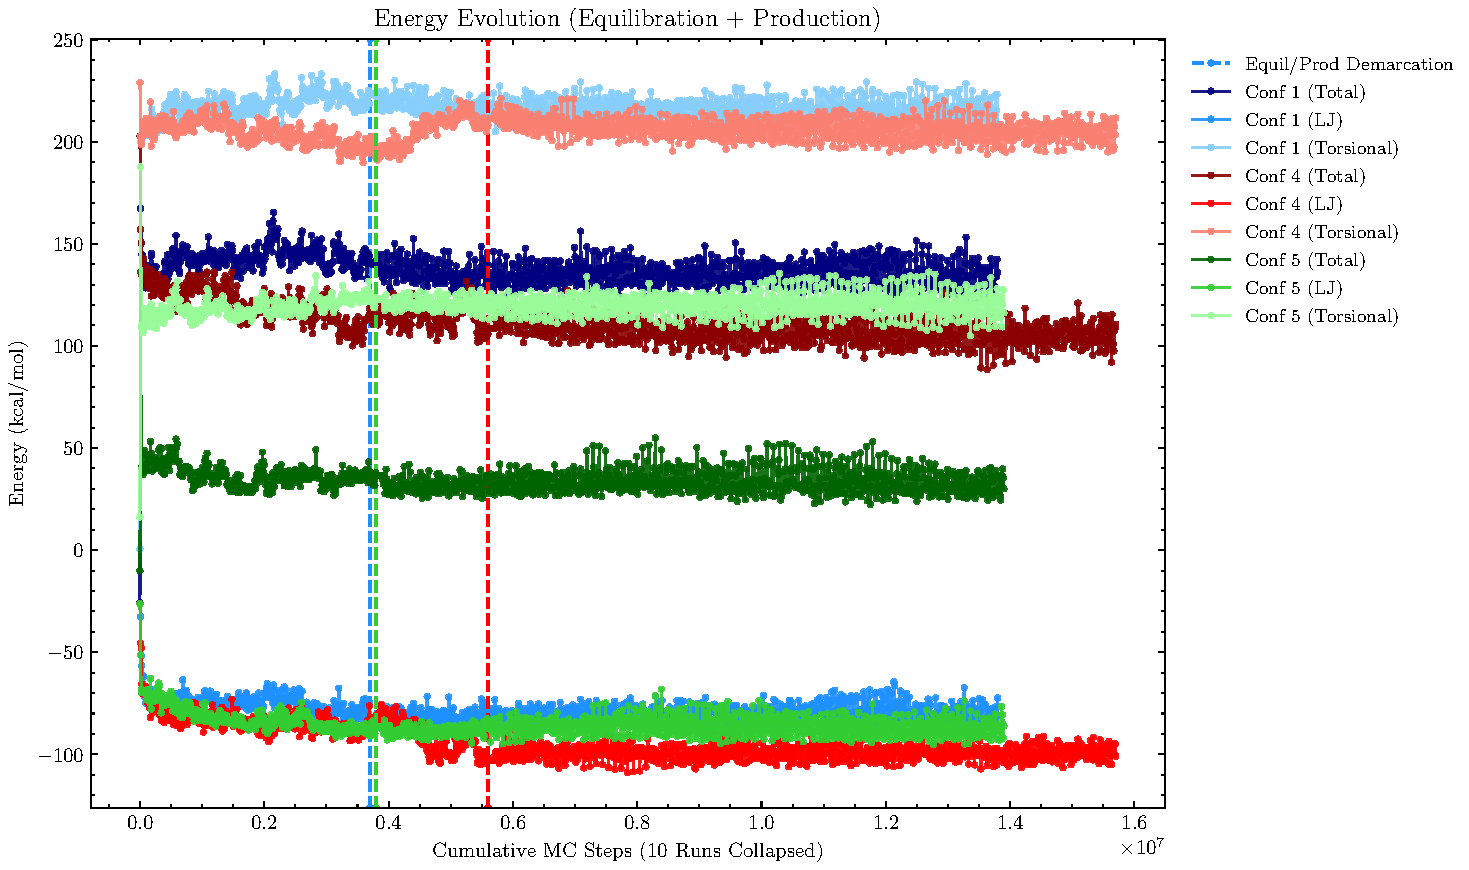
\includegraphics[width=0.8\textwidth]{figs/parallel_combined/parallel_energy_evolution.pdf}
  \caption{Total, LJ, \& Torsional Energy plots across various initial
    conformations}
  \label{fig:par_energy}
\end{figure}

Figure \ref{fig:par_energy} tracks the total, Lennard-Jones (LJ), and torsional energy
trends over the progression of Monte Carlo Steps (MCS) for
configurations 1, 4, and 5. The vertical dashed lines mark the
transition point between equilibration and the subsequent 10-million
step production data. 

In this particular instance of the combined
simulation, the torsional and LJ energy took longer to stabilize in
configuration 4 than the other configurations (1 \& 5), meaning
equilibration took longer to pass the Geweke equilibration determination
test as indicated in the red, vertical, dashed line. For this reason
its combined simultion to run for ${\sim}1.55 \times 10^7$ total steps.

An important observation and detail obtained from this graph is how
initial configuration influences the total energy within the simulation.
Configurations 1 \& 4 are rigid and straight helical structures,
respectively, while introducing random, out-of-plane tilts to
configuration 5 allowed it to find a much lower equilibrated torsional
(and therefore, total) energy.

\begin{figure}[H]
  \centering
  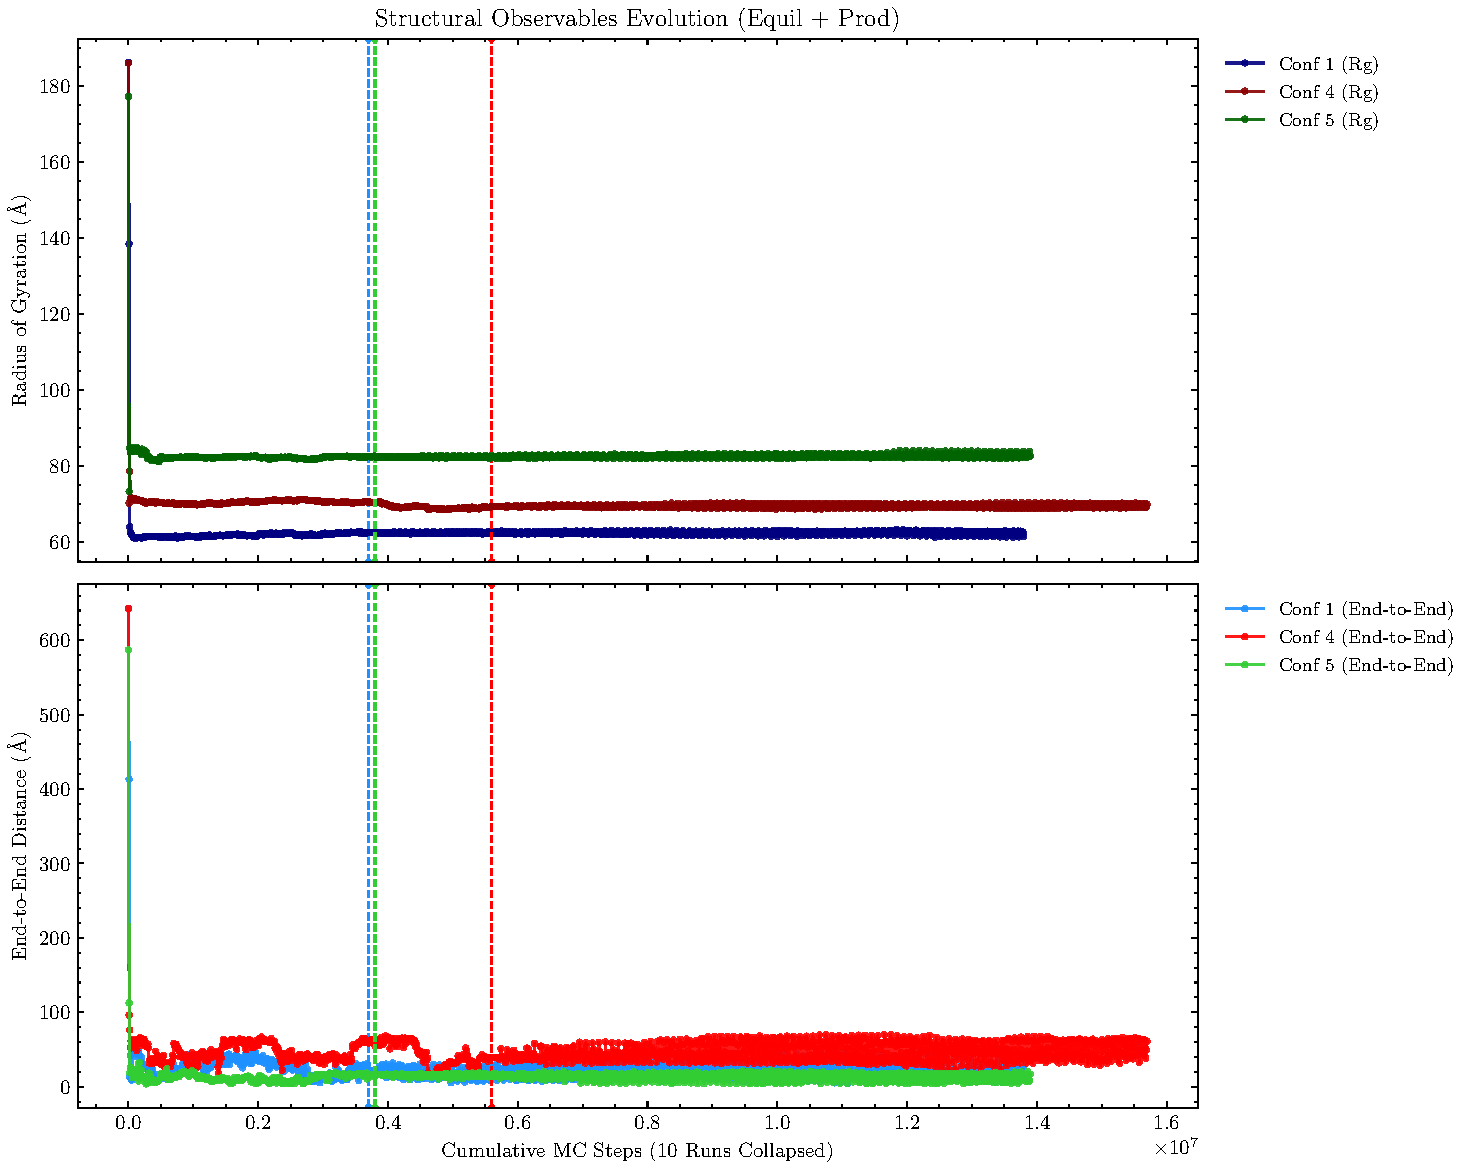
\includegraphics[width=0.8\textwidth]{figs/parallel_combined/parallel_observables_evolution.pdf}
  \caption{Radius of Gyration \& End-to-End Distance plots across
    various initial conformations}
  \label{fig:par_obs}
\end{figure}

Figure \ref{fig:par_obs} displays the Radius of Gyration (Rg) and End-to-End Distance
for the different configurations. As with the energy plots above which
showed similar torsional energies between Conf 1 \& 4 while Conf 5 was
much lower after equilibration, the Rg for Conf 5 is the most distinct
here as well. Configuration 5, due to its initial out-of-plane tilts,
was able to better relax its bonds into low-energy rotational valleys,
allowing the chain to naturally untangle and adopt an expanded, looser
geometry, mathematically resulting in a higher Radius of Gyration.

\begin{figure}[H]
  \centering
  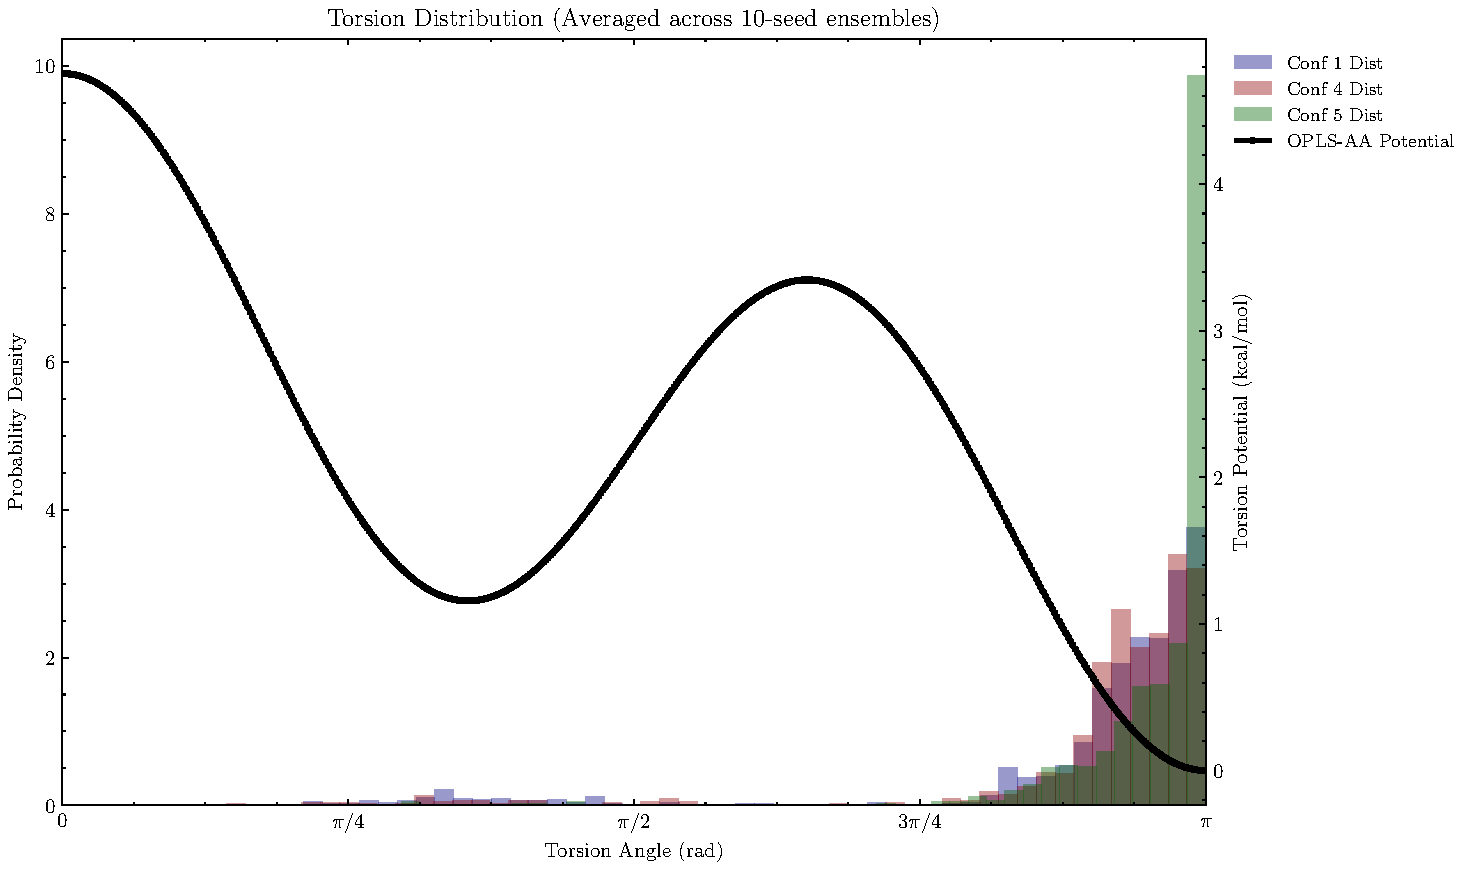
\includegraphics[width=0.8\textwidth]{figs/parallel_combined/parallel_torsion_distribution.pdf}
  \caption{Torsional distribution of post-equilibrated MCS across
    various initial conformations}
  \label{fig:par_torsion}
\end{figure}

The low-energy rotational valley relaxation tendency for Conf 5 is even
more apparent in figure \ref{fig:par_torsion}, which shows the probability density of the
each polymer exploring various dihedral (torsion) angles. Each
configuration's post-equilibration data is compared to the OPLS-AA
potential, where the results confirm the highest probability at $\pi$
(trans) configuration. While all configurations follow the expected
potential, Conf 5 adheres most closely, fully affirming the above energy
and observable data. Also of note is how the graph demonstrates the
expected rise in probablity around the potential's local minima at
${\sim}\pi/3$.